\documentclass{article}

\usepackage[latin1]{inputenc}
\usepackage[english]{babel}
\usepackage{algorithm}
\usepackage{algpseudocode}  % pseudocode (aus algorithmixs)
\usepackage{graphicx}
\usepackage{amsmath}


\newcommand{\latfit}{\textsc{LatFit}}
\newcommand{\CA}{$C_\alpha$}

\title{\latfit{} - Manual}

\date{}

\author{Martin Mann - University Freiburg \\\\
{http://www.bioinf.uni-freiburg.de/}}

\begin{document}

\maketitle


\begin{center}
  \textsc{LatPack} Tools Package
  
  Version 1.9.1
\end{center}


\section{Description}

\latfit{} allows the conversion of a protein's full atom structure
representation in Protein Data Bank (PDB) format into a coarse grained lattice
model representation. This is done by
 
\begin{enumerate}
  \item fitting the \CA-atoms to neighbored lattice positions for
  representation of the protein backbone.
  \item If side chains are modelled, $C_\beta$ or the center of mass of the
  residues are fitted to neighbored positions of the corresponding \CA{}
  atoms.
\end{enumerate}

\begin{figure}[H]
\begin{center}
	\begin{minipage}{0.4\textwidth}
		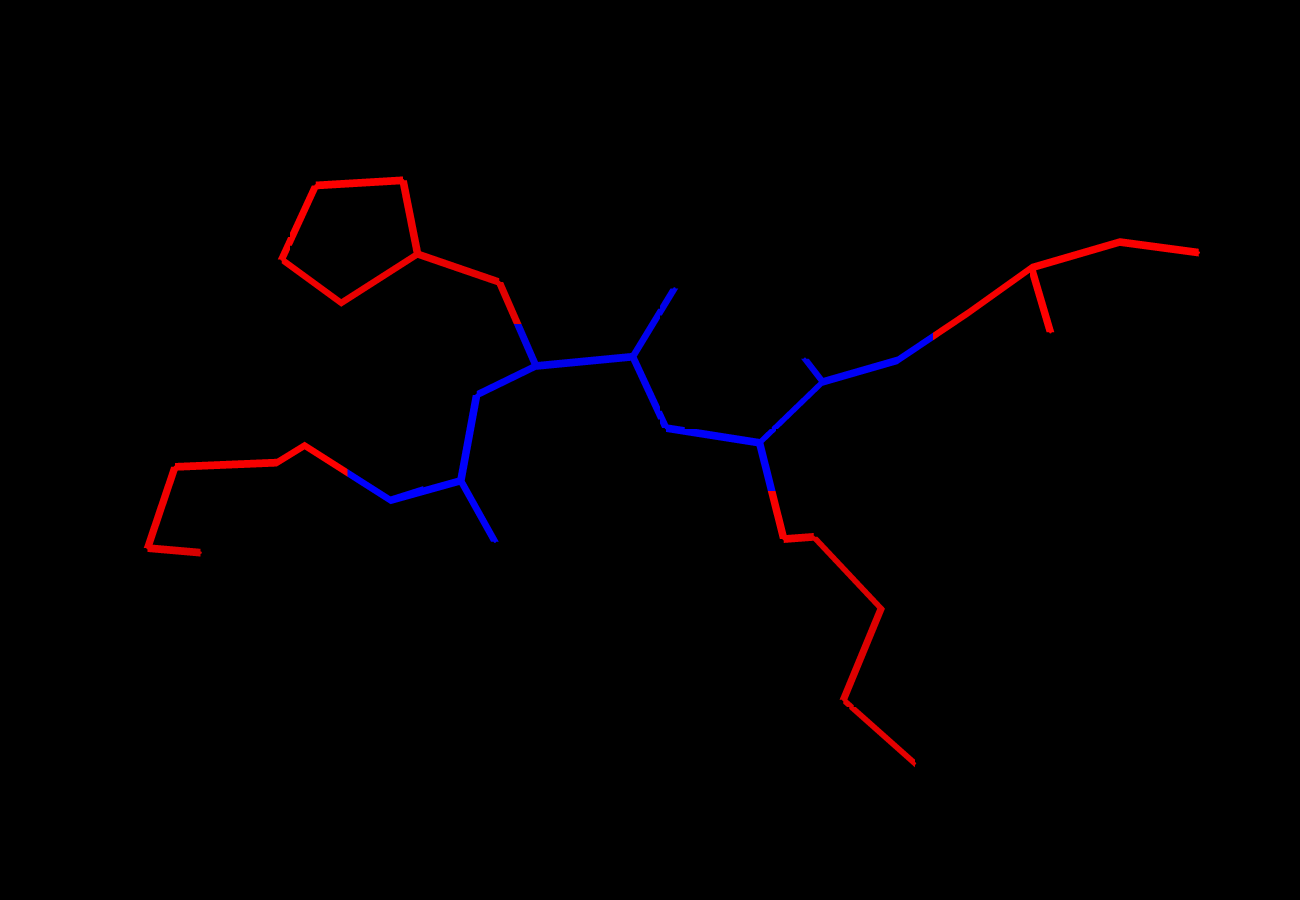
\includegraphics[width=\textwidth]{fit_pdb}
	\end{minipage}
	\begin{minipage}{0.4\textwidth}
		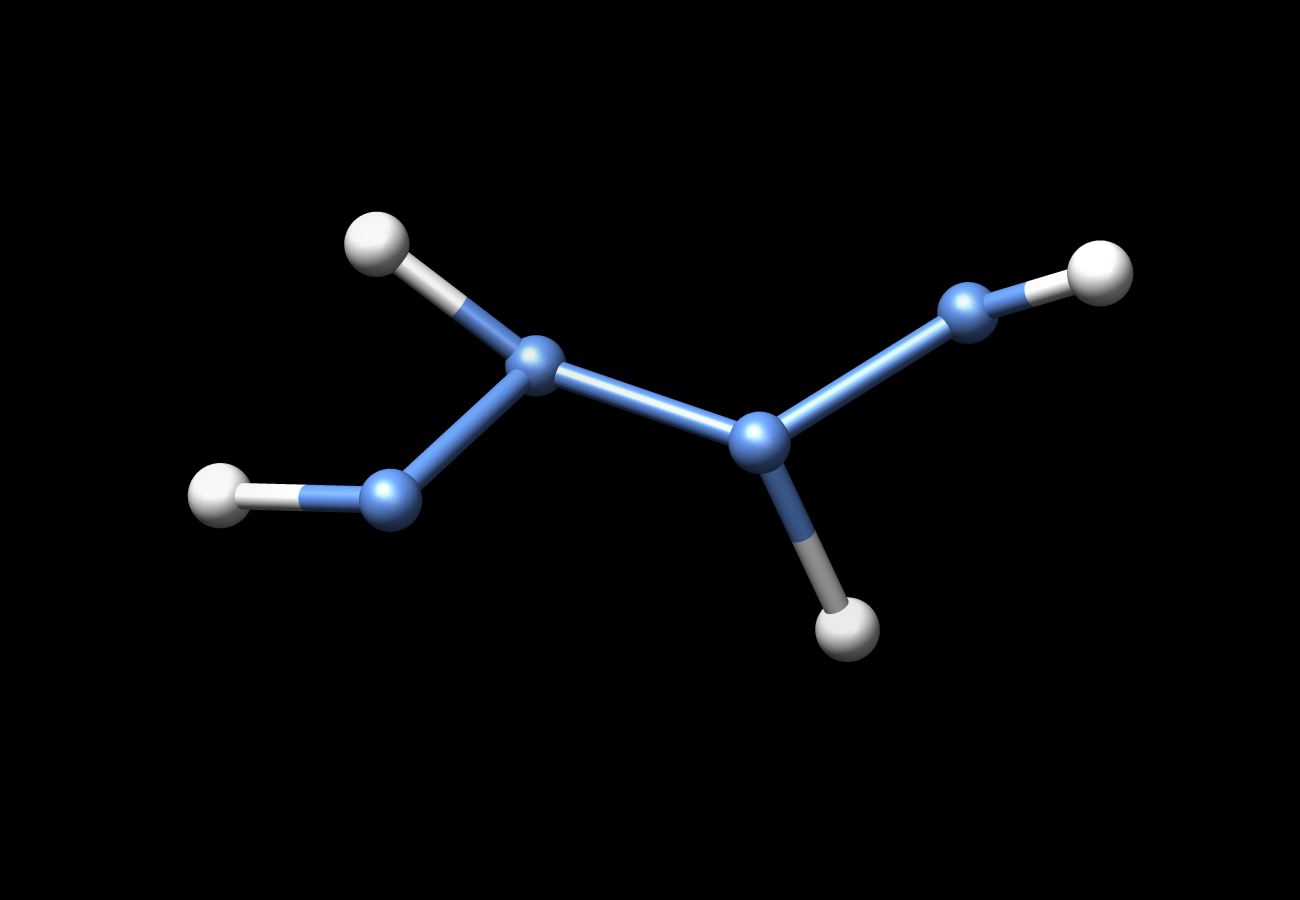
\includegraphics[width=\textwidth]{fit_lat_sc}
	\end{minipage}
\end{center}
\caption{A full atom representation of amino acids and the corresponding side
chain lattice model representation. The backbone is given in blue.}
\label{fig:pdb-lat}
\end{figure}

\vspace{0.5em}
\latfit{} implements two greedy heuristics to find the best lattice model of a
given protein utilizing the root mean square deviation (RMSD see \ref{sec:RMSD})
of a partial fit to the initial structure. The first strategy optimizes the
symmetry independent distance RMSD (dRMSD) and is given in
Sec.~\ref{sec:fit:dRMSD}. The second approach given in~\ref{sec:fit:cRMSD}
optimizes the coordinate RMSD (cRMSD), which was successfully applied in
literature
\cite{Park_Levitt:JMB:latFit:95,Miao.et.al:JMB:H-collapse:04,Godzik.et.al:JCC:globLat:93}.
Both heuristics do not ensure to find the optimal fit onto the lattice but a
reasonable good one. For instance, using the Face Centered Cubic (FCC) lattice an
approximation of the backbone with a dRMSD of 1.4~Angstroms is achieved.

\vspace{1em}
\begin{figure}[H]
\begin{center}
	\begin{minipage}{0.4\textwidth}
		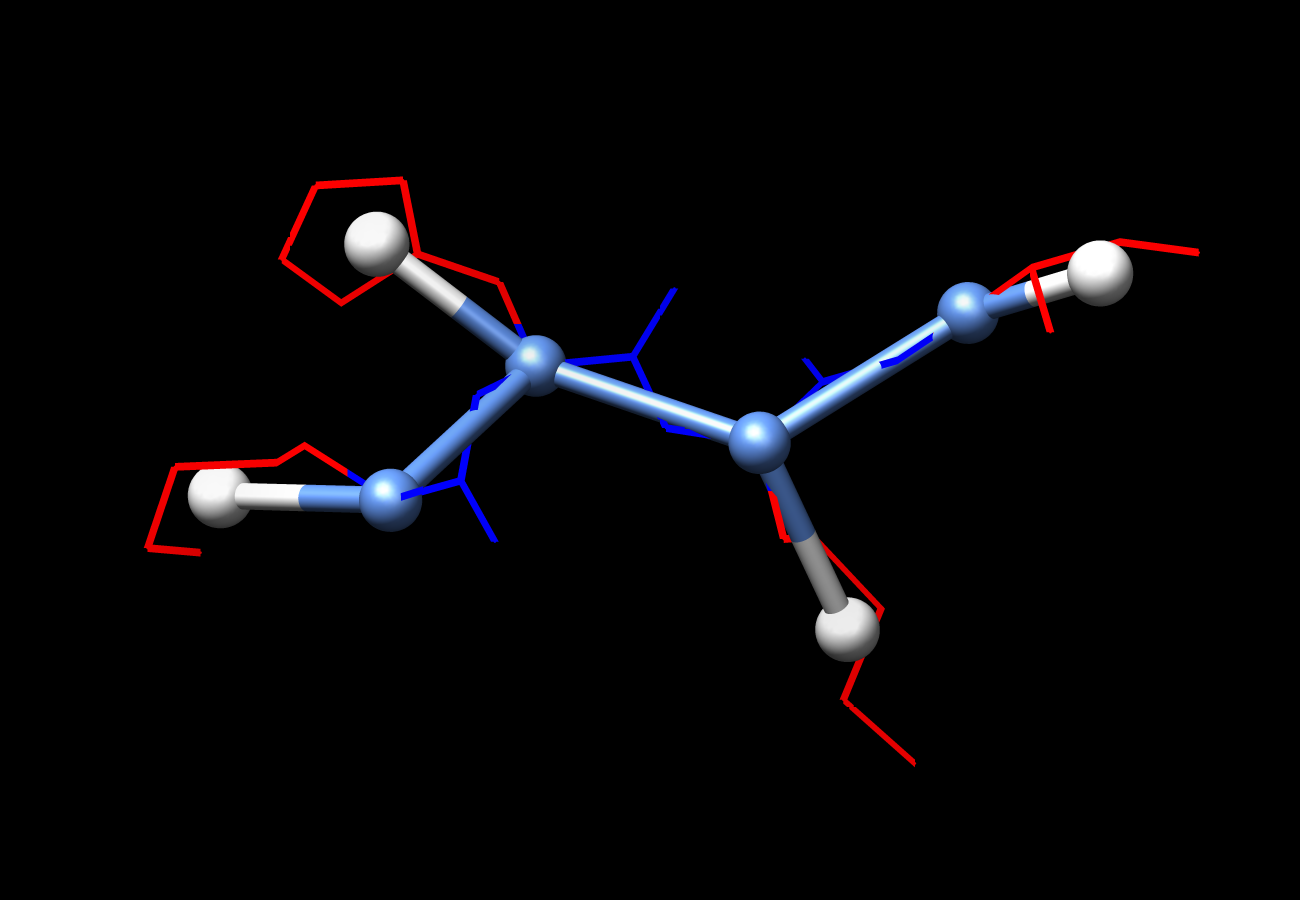
\includegraphics[width=\textwidth]{fit_both}
	\end{minipage}
\end{center}
\caption{Mapping of the full atom and lattice model structure from Fig.~\ref{fig:pdb-lat}.}
\label{fig:fit}
\end{figure}

\section{Method}
\label{sec:method}

\subsection{RMSD Definitions}
\label{sec:RMSD}

\paragraph{Backbone Models:}

The used coordinate (Eqn.~\ref{BB_cRMSD}) and distance (Eqn.~\ref{BB_dRMSD})
RMSD:

{
\begin{eqnarray}
	cRMSD & = &
	\sqrt{\frac{\sum^{l}_{i=1}
		(|\hat{P}^b_i-L^b_i|)^2}{l}} \label{BB_cRMSD}
	\\
	dRMSD & = &
	\sqrt{\frac{\sum^{ l-1}_{i=1}\sum^{l}_{j=i+1}
		(|\hat{P}^b_i-\hat{P}^b_j|-|L^b_i-L^b_j|)^2 
	}{(l \cdot (l-1))/2}} \label{BB_dRMSD} 
\end{eqnarray}
}

where $\hat{P}^b_i$ and $L^b_i$ denote the $i$th $b$ackbone coordinates of the 
rotated protein and the lattice fit of length $l$, respectively.


\paragraph{Side Chain Models:}

The used coordinate (Eqn.~\ref{SC_cRMSD}) and distance (Eqn.~\ref{SC_dRMSD})
RMSD:

{
\begin{eqnarray}
	cRMSD & = &
	\sqrt{\frac{\sum^{l}_{i=1}
		(|\hat{P}^b_i-L^b_i|)^2 + (|\hat{P}^s_i-L^s_i|)^2 
	}{2 \cdot l}} \label{SC_cRMSD}
	\\
	dRMSD & = &
	\sqrt{\frac{\sum^{(2\cdot l)-1}_{i=1}\sum^{2\cdot l}_{j=i+1}
		(|\hat{P}_i-\hat{P}_j|-|L_i-L_j|)^2 
	}{l \cdot ((2\cdot l)-1)}} \label{SC_dRMSD} 
\end{eqnarray}
}

where $\hat{P}^{b,s}_i$ and $L^{b,s}_i$ denote the $i$th $b$ackbone and $s$ide
chain coordinates of the rotated protein and the lattice fit of length $l$,
respectively, $\hat{P}=\hat{P}^s \cup \hat{P}^b$, and $L=L^s \cup L^b$.



\subsection{Lattice scaling}
\label{sec:lattice-scaling}


To enable a reasonable RMSD evaluation of the structural distance it is
important to scale the distances in the lattice to appropriate lengths. Since
all lattice protein models represent the \CA-atom of each amino acid, a scaling
based on the average \CA-distance is often applied. This distance is about
3.8~Angstroms on average in real protein structures. Thus, before applying our
fitting procedure, all neighboring vectors of the lattice are scaled to this
(user defined) length. This ensures, that the final lattice fit can be
superpositioned to the real initial protein structure. Furthermore, all
calculated coordinate and distance RMSD values are therefore in Angstroms as
well.



\subsection{Fitting : optimizing distance RMSD}
\label{sec:fit:dRMSD}

\subsubsection*{Given:}

\begin{tabular}{rcl}
	$P=P_1,\ldots,P_n$ &:& 3D coordinates of the original atoms to approximate \\
	$N$ &:& the neighboring vectors of the lattice model to use \\
	$k$ &:& number of best substructures to store per iteration
\end{tabular}

\subsubsection*{Result:}

\begin{tabular}{rcl}
	$L=L_1,\ldots,L_n$ &:& 3D coordinates of the best fit onto the lattice
\end{tabular}

\subsubsection*{Method:}

The approximation follows a greedy structure-elongating approach:

\vspace{0.5em}
\begin{algorithmic}[1]
	\State $B \gets \{k$ best fits of $P_1\}$ \Comment{best structure fits of last
	iteration} \Statex \Comment{initialized with the $k$ best fits of first
	monomer}
	\State $C \gets \emptyset$ \Comment{structures generated in current iteration}
	\For{$i = 2 \ldots n$}
		\ForAll{$L \in B$} \Comment{$L$ has length $(i-1)$}
			\ForAll{$\vec v \in N$}
				\If{$L_{(i-1)} + \vec v \not\in L_1,\ldots,L_{(i-1)}$} 
				\Comment{selfavoidingness}
					\State $C \gets C \cup \{(L_1,\ldots,L_{(i-1)},L_{(i-1)} + \vec v)\}$
					\Comment{store elongation}
				\EndIf
			\EndFor
		\EndFor
		\State $B \gets $ best $k$ fits of $C$ according to dRMSD to
		$P_1,\ldots,P_{i}$ 
		\State $C \gets \emptyset$ \Comment{reset structure storage}
	\EndFor
	\State report best fit $L \in B$ according to cRMSD to $P$
\end{algorithmic}

\vspace{1em}
{\bfseries Note:} Since the dRMSD is based on a simple sum of distances
(see~\ref{sec:RMSD}), no full dRMSD computation has to be done in line~11. It is
sufficient to update the dRMSD of the elongated fit ($L_1,\ldots,L_{(i-1)}$) with
the sum of distance differences of the appended monomer~$L_i$ to
$L_1,\ldots,L_{(i-1)}$ compared to the orginal chain. This reduces the time
complexity for each dRMSD evaluation from $O(n^2)$ to $O(n)$.

{\bfseries Note:} In order to calculate the cRMSD of the final fit, we have to
calculate a superpositioning of the lattice fit and the original data. We apply
the algorithm introduced by Kabsch~\cite{Kabsch:76,Kabsch:78} onto
all symmetric structures of the best fit found. The best superpositioning gives
the final cRMSD of the dRMSD optimized lattice fit. 



\subsection{Fitting : optimizing coordinate RMSD}
\label{sec:fit:cRMSD}

\subsubsection*{Given:}

\begin{tabular}{rcl}
	$P=P_1,\ldots,P_n$ &:& 3D coordinates of the original atoms to approximate \\
	$N$ &:& the neighboring vectors of the lattice model to use \\
	$r^X, r^Y, r^Z$ &:& rotation of the lattice according to X,Y, and Z-axis\\
	$k$ &:& number of best substructures to store per iteration
\end{tabular}

\subsubsection*{Result:}

\begin{tabular}{rcl}
	$L=L_1,\ldots,L_n$ &:& 3D coordinates of the best fit onto the lattice
\end{tabular}

\subsubsection*{Method:}

The approximation follows a greedy structure-elongating approach:

\vspace{0.5em}
\begin{algorithmic}[1]
	\State $N'\gets N$ rotated by the angles $r^X, r^Y, r^Z$
	\Comment{lattice rotation}
	\State $B \gets \{k$ best fits of $P_1\}$ \Comment{best structure fits of last
	iteration} \Statex \Comment{initialized with the $k$ best fits of first
	monomer}
	\State $C \gets \emptyset$ \Comment{structures generated in current iteration}
	\For{$i = 2 \ldots n$}
		\ForAll{$L \in B$} \Comment{$L$ has length $(i-1)$}
			\ForAll{$\vec v \in N'$}
				\If{$L_{(i-1)} + \vec v \not\in L_1,\ldots,L_{(i-1)}$} 
				\Comment{selfavoidingness}
					\State $C \gets C \cup \{(L_1,\ldots,L_{(i-1)},L_{(i-1)} + \vec v)\}$
					\Comment{store elongation}
				\EndIf
			\EndFor
		\EndFor
		\State $B \gets $ best $k$ fits of $C$ according to cRMSD to
		$P_1,\ldots,P_{i}$ 
		\State $C \gets \emptyset$ \Comment{reset structure storage}
	\EndFor
	\State report best fit $L \in B$ according to cRMSD to $P$
\end{algorithmic}

\vspace{1em}
{\bfseries Note:} Since the cRMSD is based on a simple sum of distances
(see~\ref{sec:RMSD}), no full cRMSD computation has to be done in line~12. It is
sufficient to update the cRMSD of the elongated fit ($L_1,\ldots,L_{(i-1)}$) with
the distance of the appended monomer~$L_i$ to the orginal point~$P_i$. This
reduces the time complexity for each cRMSD evaluation from $O(n)$ to $O(1)$.

{\bfseries Note:} Due to the greedy storing of the $k$ best structures only, it
may occur that none of the $k$ best of the last iteration can be extended in a
selfavoiding way (Line~6 gives 'false'). Therefore, $B$ would get empty and the
approximation stops without finding a selfavoiding fit of the whole structure
$P$. This problem can usually be solved by increasing $k$ but to the cost of
additional computations and runtime.

\subsubsection{Lattice Rotation}
\label{sec:rot}

To find the best lattice approximation of a full atom protein structure $P$ not
only one lattice orientation has to be considered. Different rotations of
the lattice along the X, Y, and Z-axis have to be generated during the search
for an optimal fit. For each rotation tuple $(r^X, r^Y, r^Z)$, the best possible
fit can be obtained using the method introduced in Sec.~\ref{sec:fit:cRMSD}.

A systematic search can be done that divides evenly a given rotation range
$[0,m\cdot\pi]$ into $s$ values for each of the rotation angles $r^X, r^Y,$ and
$r^Z$, with $m>0$ as a user defined maximal rotation factor. Afterwards, all
$s^3$ different rotation combinations are used to find the best structure
approximation. This yields the best fit $L$ of structure $P$ onto a lattice
with the corresponding best rotation angles $r^X_b, r^Y_b,$ and $r^Z_b$.

The symmetry of the lattice gives directly a maximal rotation factor $m$
necessary. For instance in the cubic lattice, a rotation of $90^{\circ}$ is
symmetric according to all axes. Therefore, $m$ can be limited to $0.5$ to avoid
unnecessary calls of the fitting procedure for symmetric rotation angles. The
same hold for the cubic and face centered cubic lattice.


\subsubsection{Refinement}
\label{sec:ref}

The best structure found via systematic search is usually not the best possible
due to the discretized rotation steps and the large size of the interval
searched. Here, a refinement of this structure can help.

Therefore, a small interval around each of the so far best rotation angles
$r^i_b \in \{r^X_b, r^Y_b, r^Z_b\}$ is defined. For a user given
refinement rotation factor $m_r>0$ the intervals are $[r^i_b-(m_r\cdot\pi),
r^i_b+(m_r\cdot\pi)]$. Once again, a systematic search is performed by an even
division of the interval in $s_r$ values. This results in additional $s_r^3$
calls of the fitting procedure.


\subsection{Glycin Handling in Side Chain Models}
\label{sec:glycin}

Glycine (GLY or G) is the smallest and simplest amino acid found in proteins.
Its chemical formula H$_2$N-CH$_2$-COOH reveals the missing side chain at the
\CA{} atom. This is no problem when fitting backbone models but for side chain
models a special handling has to be defined. Here, no distinguishing between
different amino acid structures is done and each has to be represented with two
monomers. Thus, we have to introduce a dummy side chain for Glycine as well for
which a coordinate to fit has to be set.

We decided to fit both, the backbone and the side chain monomer, of a glycin
lattice protein equivalent onto the \CA-position of the original Glycine. Thus
no artificial 'original' side chain position has to be set and the RMSD
deviation should be relatively small.


\clearpage
\section{Available Lattices}
\label{sec:lat}

Several lattice models can be used to fit a structure onto. For side chain
models, a combination of two different lattices can be used (see parameter
\mbox{\bfseries -scLat}).

\vspace{0.5em}
The currently supported lattice models and the corresponding neighboring
vectors are:

\vspace{0.5em}
\begin{tabular}{c|l|c|c}
	ID & Name & Neighborhood vectors & \#\\
	\hline
	SQR & Square & $\{\pm(1,0,0),\pm(0,1,0)\}$ & 4
	\\
	CUB & Cubic & $\{\pm(1,0,0),\pm(0,1,0),\pm(0,0,1)\}$ & 6
	\\
	FCC & Face Centered Cubic & 
	$\left\{\pm(1,1,0),\pm(1,0,1),\pm(0,1,1), \atop
	\pm(1,-1,0),\pm(1,0,-1),\pm(0,1,-1)\right\}$ & 12 
	\\
	210 & Chess Knights Walk & 
	\tiny
	$\left\{\begin{matrix}
	\pm(2,1,0),\pm(2,-1,0),\pm(2,0,1),\pm(2,0,-1), \\
	\pm(1,2,0),\pm(-1,2,0),\pm(0,2,1),\pm(0,2,-1), \\
	\pm(1,0,2),\pm(-1,0,2),\pm(0,1,2),\pm(0,-1,2)\\
     \end{matrix} \right\}$ & 24 
	\\
\end{tabular}

\section{Program Parameters}

\subsubsection*{\underline{ PDB Input }}

\begin{description}
	\item[-pdbFile] The full atom protein representation to fit onto a
	lattice in Protein Data Bank (PDB) format. If this parameter is not given or
	set to 'STDIN', the structure is read from the standard input.
	\newline\emph{Note:} \mbox{\bfseries -fitSideChain} is used, reading from
	'STDIN' is not possible due to a necessary double parsing of the PDB input.
	\item[-pdbAtom] The atom identifier that has to be fitted as the backbone
	monomer of the lattice structure. Usually, 'CA' for \CA-atoms is used.
	If 'CoM' is given, the center of mass of the amino acid side chain is
	fitted. If \mbox{\bfseries -fitSideChain} is used, the given atom is fitted as
	the side chain monomer of the structure and \CA{} for the backbone. 
	\item[-pdbAtomAlt] If the PDB file contains alternatives for atoms to fit, an
	alternative identifier has to be given to allow a unique fit.
	\item[-pdbChain] In case the PDB file contains several amino acid chains, one
	chain to process has to be specified.
	\item[-pdbChainGaps] Some PDB files show imcomplete atom position information
	such that no information is given for some amino acids. Such \emph{gaps} in
	the sequence are usually rejected by the program that tries to fit an entire
	chain. If such a non-consecutive chain with gaps should be fitted instead, the
	parameter \mbox{\bfseries -pdbChainGaps} has to be given.
\end{description}


\subsubsection*{\underline{ Lattice Settings }}

\begin{description}
	\item[-lat] The lattice onto that the backbone has to be fitted. The
	available list of lattice identifiers is given in Sec.~\ref{sec:lat}.
	\item[-bondLength] The distance in Angstroms between two neighbored
	\CA-atoms in the lattice. Used to scale all neighboring vectors of the
	lattice (Sec.~\ref{sec:lat}) to this length. For default we suggest the common
	value~'3.8' used in literature.
\end{description}


\subsubsection*{\underline{ Side Chain Settings }}

\begin{description}
	\item[-fitSideChain] If present, a fit of two monomers per amino acid is done.
	One for backbone and one representing the side chain. The \CA-atom ('CA')
	is used to fit the backbone monomer. The atom specified with \mbox{\bfseries
	-pdbAtom} is used for the side chain monomer fit.
	\newline{\bfseries Note:} The fit of a Glycine amino acid 
	includes a side chain monomer as well, even it has none in real proteins!
	Here, both monomers (backbone and side chain) approximate the \CA-atom
	position.
	\item[-scLat] Per default the same neighboring vectors as for the backbone fit
	(\mbox{\bfseries -lat}) are used for the neighboring of backbone
	(\CA) and side chain monomers. Using \mbox{\bfseries -scLat}, a different
	set of allowed neighboring vectors (=lattice) can be specified. The length of
	these vectors are calculated in relation to the backbone vector lengths 
	(see \mbox{\bfseries -bondLength}). The
	available list of lattice identifiers is given in Sec.~\ref{sec:lat}.
	\item[-scContrib] Allows for a weight of the side chain fit according to the
	backbone approximation. This factor is multiplied to each side chain monomer
	RMSD that is added to the overall RMSD. Therefore, higher the value yield
	a better fit of the side chain monomer compared to the \CA{} atom.
	\newline{\bfseries Note:} a value $\not = 1.0$ makes the reported RMSD
	meaningless due to the scaling of the side chain distances!
	\item[-fitDirVec] If present, a fit of direction vectors instead of side chain
	atoms is performed. A
	direction vector is given by \mbox{$\vec{d}=k\cdot(\textbf{pdbAtom}-C_\alpha)$}, whereby $k$ is a calculated
	scaling factor to set the length of $\vec{d}$ to \mbox{\bfseries dirVecLength}.
	\item[-dirVecLength] The length of the direction vector to fit, if
	\mbox{\bfseries -fitDirVec} is specified.
\end{description}


\subsubsection*{\underline{ Fitting Parameters } (see Method
Sec.~\ref{sec:method})}

\begin{description}
	\item[-optMode] Defines what optimization strategy to use :
		\begin{description} 
			\item[\texttt{D} :] distance RMSD (see~\ref{sec:fit:dRMSD}) [default]
			\item[\texttt{C} :] coordinate RMSD (see~\ref{sec:fit:cRMSD})
		\end{description} 
\end{description}

The following parameters apply to the coordinate RMSD optimization only
(see~\ref{sec:fit:cRMSD}):

\begin{description}
	\item[-rotMax] Factor that limits the maximal rotation angles in radian
	measure. The rotations are done within $[0.0, \textbf{rotMax}\cdot\pi]$ for
	each dimension X,Y, and Z.
	\item[-rotSteps] Number of discrete rotation steps done to find a good fit.
	Therefore, the interval $[0.0, \textbf{rotMax}\cdot\pi]$ is divided into
	{\bfseries rotSteps} equal intervals.
	\item[-nKeep] Number of best structures to store that are extended in the next
	iteration.
	\item[-refRotSteps] Determines if a refinement of the best structure of the
	``global'' screening should be done or not. If set to~0 no refinement is done.
	Otherwise, the best approximation should be improved. This is done via a
	fine grained rotation around the best angles $r^X, r^Y, r^Z$ so far. The
	rotation is done in the intervals $[r^i-\Delta r, r^i+\Delta r]$ around
	each rotation angle with $i\in\{X,Y,Z\}$ and $\Delta r =
	\textbf{refRotMax}\cdot\pi$.
	\item[-refRotMax] Factor that defines the rotation intervals around the best
	rotation angles so far in which a refinement should be done (see {\bfseries
	-refRotSteps}).
\end{description}


\subsubsection*{\underline{ Output }}

\begin{description}
	\item[-outMode] The format in that the output should be written. Possible
	formats are: \newline
	\begin{minipage}{0.6\textwidth}
    \vspace{1em}
	\begin{tabular}{c|l}
    	ID & Format Description \\
    	\hline
    	CML & Chemical Markup Language (XML) \\
    	PDB & Protein Data Base format\\
    	XYZ & Coordinate output (plain text) 
    \end{tabular}
	\end{minipage}
	\item[-outFile] If not specified or set to 'STDOUT' the final structure output
	is done to standard output. Otherwise it is written to the specified file.
	\item[-outAllBest] Every time a better fit than the last best found is achieved
	the corresponding structure is printed.
	\item[-outLatPoint] Prints the non-rotated lattice structure with discrete
	lattice positions instead of the rotated. 
	\newline{\bfseries Note:} Also the neighbor vector scaling via \mbox{\bfseries
	\mbox{-bondLength}} is ignored!
	\item[-outOrigData] If present, adding the atom positions of the original
	protein structure ({\bfseries \mbox{-pdbFile}}) to the output.
\end{description}


\subsubsection*{\underline{ Miscellaneous }}

\begin{description}
	\item[-v] Give verbose output during computation.
	\item[-s] Give only minimal output during computation.
	\item[-help] Prints the available program parameters.
\end{description}


\section{Contact}

\begin{tabular}{lcr}
	Martin Mann  && \bfseries http://www.bioinf.uni-freiburg.de/\\
	Bioinformatics Group\\
	University Freiburg, Germany \\
\end{tabular}





\begin{thebibliography}{99}
\bibitem{Park_Levitt:JMB:latFit:95}{
	  B.~H.~Park and M.~Levitt:
	  {\bfseries The Complexity and Accuracy of Discrete State Models of Protein
	  Structure}, \emph{Journal of Molecular Biology} 1995,
	  {\bfseries 294}:493-507
	 }
\bibitem{Miao.et.al:JMB:H-collapse:04}{
	  J.~Miao, J.~Klein-Seetharaman and H.~Meirovitch:
	  {\bfseries The Optimal Fraction of Hydrophobic Residues Required to Ensure
	  Protein Collapse}, \emph{Journal of Molecular Biology}
	  2003,
	  {\bfseries 344}:797-811
	 }
\bibitem{Godzik.et.al:JCC:globLat:93}{
	  A.~Godzik, A.~Kolinski and J.~Skolnick:
	  {\bfseries Lattice Representations of Globular Proteins: How Good Are They?},
	  \emph{Journal of Computational Chemistry} 1993,
	  {\bfseries 14(10)}:1194-1202
	 }
\bibitem{Kabsch:76}{
	W.~Kabsch: 
	{\bfseries A solution for the best rotation to relate two sets of vectors},
	\emph{Acta Crystallographica} 1976, 
	{\bfseries A32}:922-923
}
\bibitem{Kabsch:78}{
	W.~Kabsch: 
	{\bfseries A discussion of the solution for the best rotation to relate
	two sets of vectors},
	\emph{Acta Crystallographica} 1978, 
	{\bfseries A34}:827-828
}
\end{thebibliography}
 

\end{document}